\section{quantum microarchitecture}
In this section, we will discuss the electrode event-based quantum microarchitecture as shown in figure~\ref{img2}. 

The input of ebQuMA is generated by the compiler infrastructure, 
which compiles the quantum program 
(including the quantum application described by the gate model and the calibration experiment program) 
into a micro-architecture program coding with ebQIS (electrode event-base Quantum Instruction Set) as shown in table1, 
and generates the waveform file corresponding to each event. 

ebQIS is composed of classic and quantum instructions. 
Classic instructions include arithmetic and logical operations, branch, load and store instructions to support data transferring and program flow control.  
Quantum operation instruction and Qwait are used to describe the electrode events of qubits for each given timestamp, 
and FMR is necessary to obtain the measurement result of qubits. 
In order to increase the information density of the instructions, 
we refer to the VLIW(very long instruction word) and SIMQ(single instruction multiple qubits) schemes proposed by eQASM. 
A quantum operation instruction can contain up to two quantum operations. 

As shown in figure5, the instruction execution unit fetches and executes ebQIS instructions from the instruction memory, performing registers update, program flow control and data communication. 
In particular, quantum operation instructions buffer electrode events with the same timestamp into event registers and send to the queue control unit when a new timestamp arrives. 
The event controller sends the buffered events at the time point specified by the timestamp, to achieve precise time control. 
Pulse generator units obtain the size and address of the waveform according to the encoding of the electrode events, and converts digitally events into corresponding analog pulses by DACs. 
After modulating the output signal of XY feedline and measure pulse generators with radio-frequency carrier waves, 
analog pulses with precise timing can perform quantum operations on qubits. For the measure event, 
in addition to generating measurement waveform, the queue control unit sends the measurement signal to the measurement calculation unit. 
After a fixed delay, the MCU starts to collect the demodulated measurement analog signal, 
obtain the measurement result and send to the instruction execution unit.

We introduce three schemes in ebQuMA to address the challenges described in Section 4.
(i)In ebQIS, The quantum circuit is describing with electrode event based quantum operation. 
By allocating multiple electrode event registers for each qubit, ebQASM supports to apply multiple waveform on different electrode at one timestamp. 
This scheme makes calibration experiments and waveform compensation possible in ebQuMA. 
(ii)electrode events in ebQIS are divided into global and local events, which complement each other. 
The global events can greatly reduce the instruction overhead of circuit description, so as to offset the issue rate problem caused by supporting waveform compensation. 
While local events are used to discribe low gate diversity circuit with high depth to reduce the memory overhead, such as Random Benchmarking.
(iii)In order to support the above two scheme, a multi-level compilation scheme is necessary. The compilation process is divided into three steps. 
Transforming the circuit with gate model into electrode events based description scheme, 
generating waveforms corresponding to each event and micro-architecture program, 
and assigning the coding of each event according to the waveform size and storage address in ebQuMA.

\subsection{Electrode Based Quantum Operation Unit}
First, we propose independent electrode number to characterize the control architecture of different quantum processors. 
The independent electrodes number refers to the category number of independent electrodes required for each qubit to perform all quantum control operations (not including measure operation). 
If one operation requires multiple waveforms superimposed simultaneously, 
since each of them cannot independently implement one operation respectively, 
the number of independent electrodes is still 1(such as XY-rotation operation for superconducting transmon qubit). 
Table 2 shows the independent electrode number of different superconducting quantum processor. 
Although the types and implementation schemes of quantum gates varies, 
In most architecture, two independent electrodes are necessary to implement XY-rotation and Z-rotation \& two-qubit gates, respectively. 
In particular, Google's architecture additionally requires one independent electrode for the coupler.

ebQuMA adopt the electrode event, a abstraction of waveforms on one specific electrode for one qubit, as the basic unit of quantum operation in ebQIS. 
It can be one or combination of multiple quantum gates, or a waveform for calibration experiment and optimized circuit. 
The number of electrode event types depends on the independent electrode number, and distinguished by the encoding of quantum operation. 
Table 3 shows the coding of quantum operation for the quantum processor mentioned in Section 2. 
The quantum circuit in a time period for each qubit is obtained by independent description of different electrode events. 


\begin{algorithm}[ht]
      \caption{caption}
      \begin{ttfamily} 

      \textcolor[RGB]{0,0,205}{ADDI } \quad R1, R0, 40000   \qquad \textcolor[RGB]{169,169,169}{\#cycle number for each measurement}\\
      \textcolor[RGB]{0,0,205}{ADDI } \quad R5, R0, ResultMemAddr\\
      \textcolor[RGB]{0,0,205}{SMIS } \quad S0, 1\\
      \textcolor[RGB]{0,0,205}{ADDI } \quad R2, R0, 0\\
      \textcolor[RGB]{0,0,205}{ADDI } \quad R3, R0, 0\\
      ~\\
      \textcolor[RGB]{34,139,34}{Loop\_1:}\\ 
      \quad 0 , \textcolor[RGB]{139,69,19}{X\_event1} S0 | \textcolor[RGB]{139,69,19}{Z\_event0} S0\\
      \quad 3 , \textcolor[RGB]{139,69,19}{measure} S0\\
      \quad \textcolor[RGB]{0,0,205}{QWAIT} \quad 50\\
      \quad \textcolor[RGB]{0,0,205}{FMR\quad} \quad R4, S0\\
      \quad \textcolor[RGB]{0,0,205}{ADD\quad} \quad R3, R4, R3\\
      \quad \textcolor[RGB]{0,0,205}{ADDI } \quad R2, R2, 1\\
      \quad \textcolor[RGB]{0,0,205}{BNE\quad} \quad R1, R2, \textcolor[RGB]{34,139,34}{Loop\_1}\\
      ~\\
      \textcolor[RGB]{0,0,205}{STORE} \quad R5, R3\\
      \textcolor[RGB]{0,0,205}{ADDI } \quad R3, R0, 0\\
      \textcolor[RGB]{0,0,205}{ADDI } \quad R2, R0, 0\\
      \textcolor[RGB]{0,0,205}{ADDI } \quad R5, R5, 1\\
      ~\\
      \textcolor[RGB]{34,139,34}{Loop\_2:}\\
      \quad 0 , \textcolor[RGB]{139,69,19}{X\_event1} S0 | \textcolor[RGB]{139,69,19}{Z\_event1} S0\\
      \dots

      
      \end{ttfamily} 
\end{algorithm} 

Lower-level control compared with the gate model allows ebQuMA to support calibration experiments.
Figure 5a is a micro-architecture program used to calibrate the timing difference between the microwave drive and flux bias channels based on ebQIS. 
XYevent\_0 corresponds to a $\pi$ pulse and each Zevent corresponds to flattop Z detune shown in figure5b. 
The pulse duration is the same as $\pi$ pulse, while varying the timing between the two. 
The host program can obtain the timing difference from the final state probability of each Zevent and the corresponding delay.

On the other hand, the electrode event can be a waveform of one quantum gate or a combination of quantum gates, which is suitable for the description of quantum circuits with different depth. 
For the quantum circuit shown in Figure 6, we use two different levels abstraction of electrode events to describe. 
One electrode event coding scheme is to encode a combination of all quantum gates of single electrode into one electrode event, and add unitary operation waveforms when no operation applies. 
Correspondingly, the description procedure of this circuit is:\\
\centerline{0,\quad  XYevent\_1 \quad S0 \quad | \quad Zevent\_2 \quad S0;}\\
It only takes one instruction, but require to store the waveform with a total length of 120ns, which includes unitary operation waveforms and repetitive waveforms.

Also, we can take a lower level of abstraction that only encode waveforms of basic quantum gates as electrode events. 
The corresponding procedure is:\\
\centerline{0, \quad XYevent\_2 \quad S0;}\\
\centerline{2, \qquad  Zevent\_3 \quad S0;}\\
\centerline{2, \quad  XYevent\_2 \quad S0;}\\

\begin{figure}[h]
  \centering
  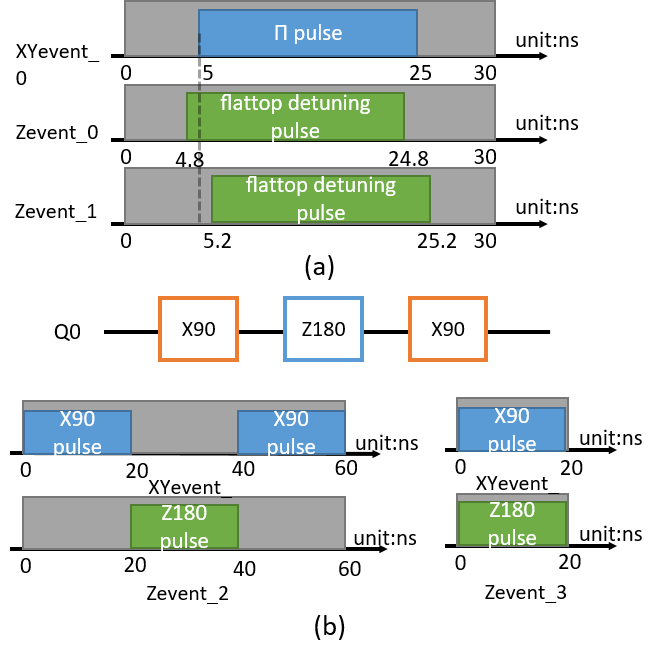
\includegraphics[width=\linewidth]{figure/4_34}
  \caption{overview of electrode event-based microarchitecture}
  \label{img4}
\end{figure}


Although it requires 3 instructions, it only needs to store the waveform of 40ns. 
High level abstraction completes more task of circuit description during the compilation phase instead of runtime, reduces instruction number horizontally
at the cost of memory overhead. The memory resource consumption of this solution will be discussed more in section 8.
In contrast, Lower level abstraction of electrode events greatly reduces memory overhead, which is suitable for the circuit with large depth, such as random benchmarking. 

To support the electrode event-based description scheme, the number of event registers and event queues for each qubit is equivalent to independent electrode number in ebQuMA. 
The instruction execution module buffers quantum operations of different electrodes for each qubit in the corresponding electrode event register when executing the quantum operation instruction, 
and sends the buffered electrode events to the corresponding electrode event queue uniformly when a new timestamp is generated. 
When the queue control unit is triggered and a certain timestamp is reached, 
all electrode events executed at this timestamp are sent to the corresponding waveform generation modules that play the pre-stored waveform synchronously according to the electrode event code.
It is worth noting that since the electrode event is an abstraction of the actual waveform, to adapt different quantum chip architectures, 
the microarchitecture only needs to modify the number of electrode event registers and queues.

\subsection{hybrid Event Description Scheme }
Although the electrode event-based quantum operation unit provides the possibility to implement calibration experiment and waveform compensation, 
it requires to specify the quantum operation applied by each electrode of each qubit for every timestamp. 
Even if we take SOMQ and VLIW schemes, for quantum circuits with large gate diversity, 
such as QV algorithms, and quantum gates required waveform compensation, 
which means every qubit needs to apply a quantum operation (quantum gate waveform or compensation waveform), 
it will still cause serious issue rate problem, especially when qubit number is large. 
To this end, we propose a hybrid event description scheme with local and global events.

The local event requires an operand in mask format to specify the target qubits. Generally, local electrode events are low-level abstractions, 
representation of single quantum gate or calibrated waveform. 
When performing quantum applications, each local event corresponds to one quantum gate, same as the gate model.
By using local event to describe quantum circuit, only basic waveforms need to be stored, but requires more instructions, which is suitable for circuits with lower gate diversity but larger depth. 
For calibration experiments, the local events of each qubit are independent of others, which means they are not valid on every qubit, specified during the compilation phase.

In addition to local events, ebQIS introduces global events, which apply the electrode event on all qubits. 
The types of events are distinguished by the coding of quantum operations, as shown in Table 1. 
Since the global event does not require an operand, the segment corresponding to the operand register is used as an extension segment for the quantum operation encoding, 
providing a larger addressing space for global events.
As all qubits need to perform global events, (no operation qubits play the unitary operation waveform), 
when the gate density is low, more invalid waveform are stored, Resulting in low memory utilization. 
However, for large gate diversity circuit, global events can greatly reduce the number of instructions and avoid issue rate problems. 
In particular, since compensation quantum gates require to apply waveforms on all qubits, they are well-suited for global event coding.

\begin{figure}[h]
  \centering
  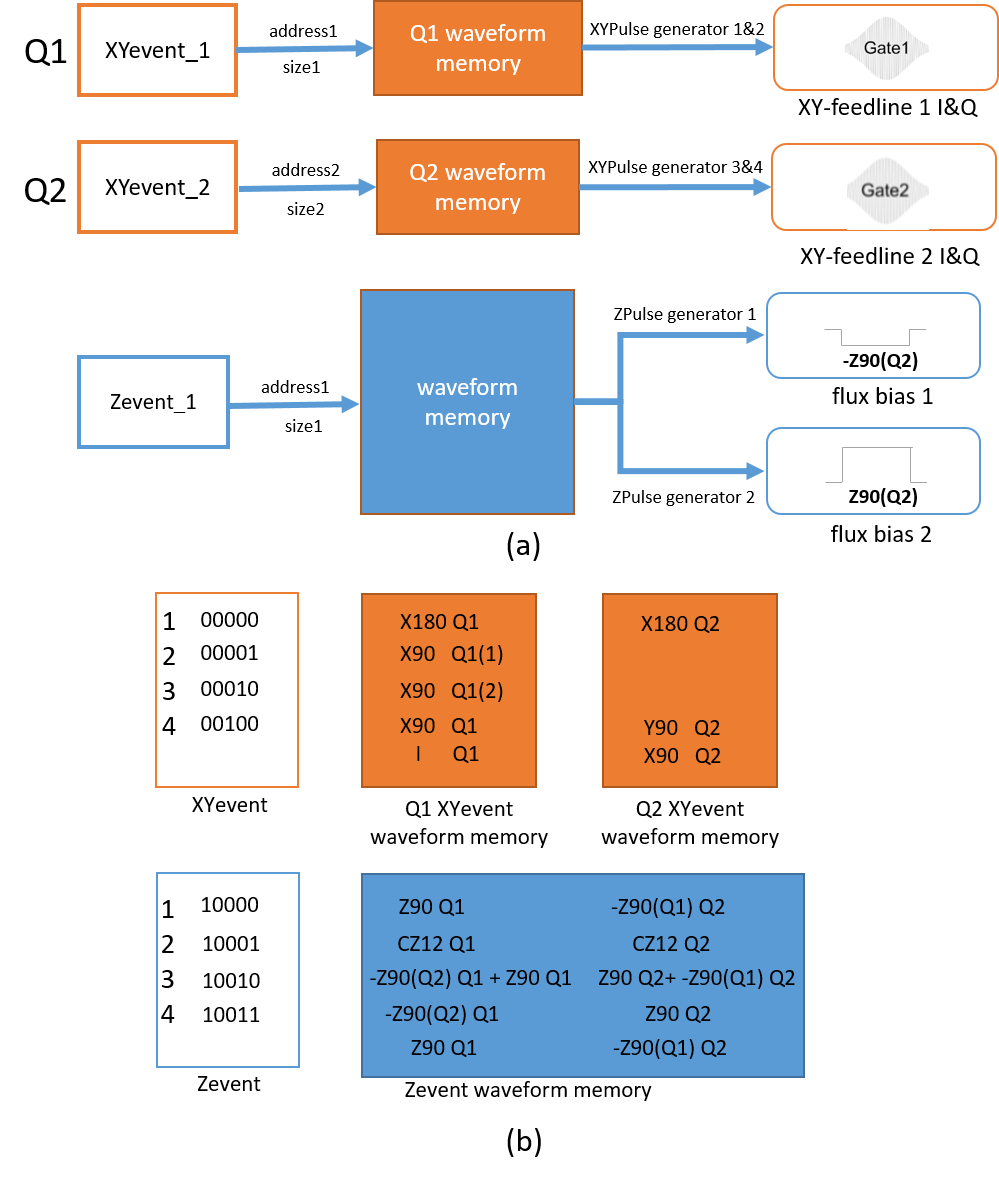
\includegraphics[width=\linewidth]{figure/4_6}
  \caption{overview of electrode event-based microarchitecture}
  \label{img6}
\end{figure}

Considering all quantum operations on the flux bias line require waveform compensation for the superconducting quantum processor as mentioned in Section 2, 
in ebQuMA, all Zevents are described by global events, reducing hardware resource overhead of local Zevent registers and queues. 
As a result, there is n local registers of XYevent and one global register of Zevent in ebQuMA where n is the qubit number. 
When a quantum instruction is executed, the instruction execution module buffers all electrode events with the same timestamp into corresponding event registers according to the event and electrode type. 
Specifically, when a global XYevent operation instruction is executed, the execution module broadcasts the event to every local XYevent register.


The pluse generator unit of ebQuMA is divided according to the electrode type. Limited by hardware resources, 
each waveform generating unit has a maximum of 8 DACs and supports the control of up to 4 qubits of XY electrode or 8 qubits of Z electrode.
The process of decoding events into waveforms and waveform memory model of XY and Zevents are shown in Figure 5. For the XY feedline pulse generator unit, 
each qubit has a separate waveform memory (about 4MB) to store three types of waveforms:
\begin{itemize}
  \item XYevent\_1 is a local event of low-level abstraction that represents single XY-plane rotation quantum gate. 
  The waveform of quantum gate for each qubit needs to be stored in respective waveform memory whose address corresponds to the event code.
  \item XYevent\_2, 3 is also a local event, which is used to represent the waveform of the calibration experiment. 
  In this example, we only calibrate waveform of X90 applied on Q1, thus waveforms only store in the waveform memory of Q1, 
  and the address corresponds to XYevent\_2,3. The waveforms of other qubits in this address space are invalid. 
  If the operand is other qubits, an error will be reported during the compilation phase.
  \item XYevent\_4 is a global event with a higher level of abstraction, which represents electrode events of all qubits in a period of time. 
  Each qubit has a waveform with the same length in the address corresponding to the global event.
\end{itemize}
The XY feedline pulse generator decodes the electrode event of each qubit received from Queue control unit to obtain the address and waveform file size of each event in its own waveform memory, 
and sends it to the corresponding DACs. Each qubit requires two DACs to play two waveforms of In Fhase and Quadrature respectively. Measure pulse generator unit works in the same way as The XY feedline pulse generator, 
except that there is no global event for the measurement.

For the flux bias pulse generator unit, 
All flux bias electrodes share single memory (about 16MB) for waveforms of global event. 
Zevents can be low-level abstractions, such as one Z-rotation gate or a CZ gate, 
corresponding to Zevent\_1,2, or quantum gates applied on different qubits for one timestamp as Zevent\_3, 
or a high-level abstraction of quantum circuits, such as Zevent\_4. When receiving new global event, 
the flux bias pulse generator unit obtains the waveform of each qubit corresponding to the event code from the waveform memory, 
and distributes the waveform file to each DAC through the pulse distribution module.

\subsection{Multi-level Compilation Scheme}

Since quantum applications are described using quantum circuits based on the GATE model, 
while ebQuMA based on electrode events, a multilevel compilation architecture is required to compile quantum applications into ebQuMA executable files. 
It should be noted that mapping between quantum circuit and processor is completed by the top-level compiler, outside the scope of this paper. 
The input circuit of our scheme is optimized and each quantum gate can be directly executed by quantum hardware.
Specifically, the compilation of quantum applications requires the following four steps, as shown in Figure:
\begin{figure}[ht]
  \centering
  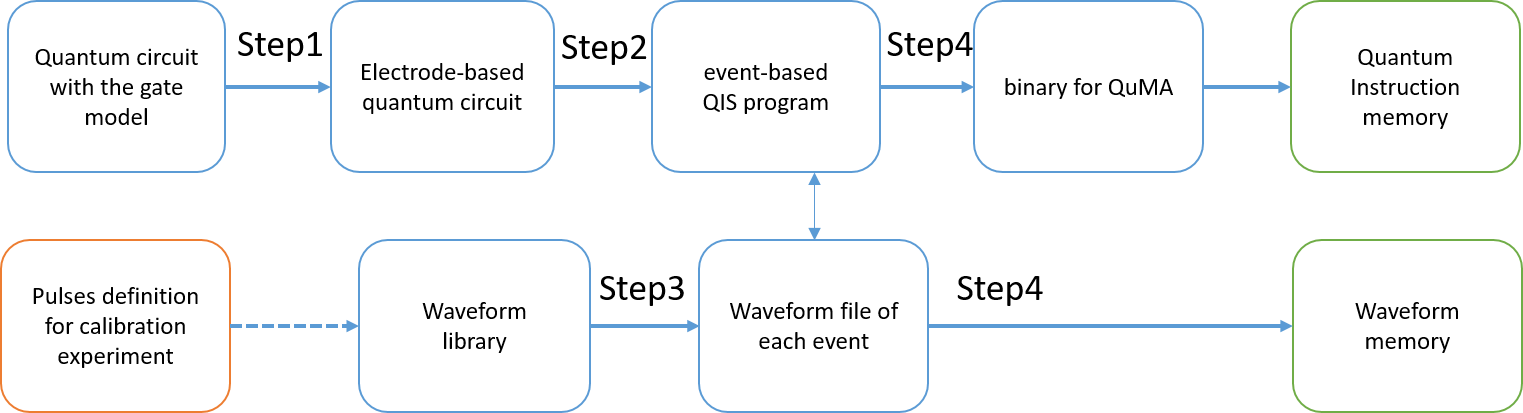
\includegraphics[width=\linewidth]{figure/4_8}
  \caption{overview of electrode event-based microarchitecture}
  \label{img7}
\end{figure}


First, the gate-based quantum circuit is divided into multiple sub-circuits each of which is implemented by one type of electrodes, independently. 
Figure 2.a is the quantum circuit of 3-qubit DJ algorithm. The H-gate is performed by applying one X90 and Z180 gate back to back. 
The circuit is split to two sub-circuits in Figure8. B according to the execution electrode. 
The left part is executed by the XY feedline to implement XY-rotation operation and right one is performed by flux bias lines for Z-rotation and CZ operations. 
I represents the unitary operation and the time axis below the circuit records the initial timestamp of each operation.
\begin{figure}[h]
  \centering
  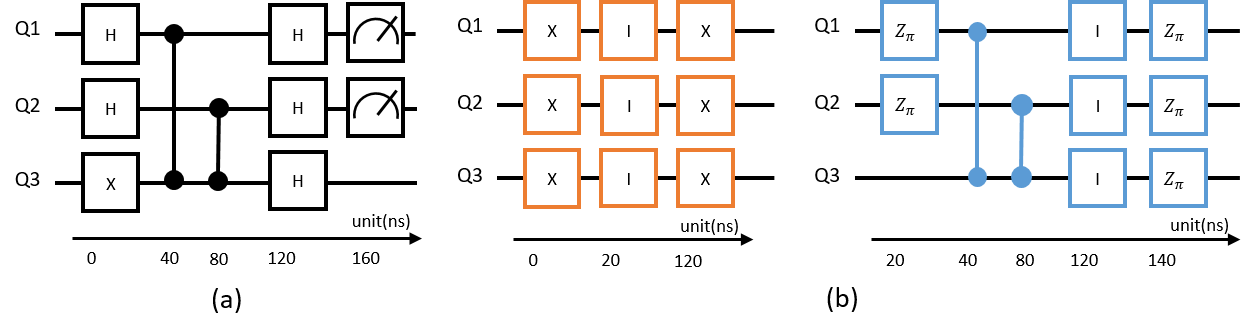
\includegraphics[width=\linewidth]{figure/4_10}
  \caption{overview of electrode event-based microarchitecture}
  \label{img7}
\end{figure}


Secondly, define electrode events with different levels of abstraction according to the characteristics of the quantum circuit for circuit description and use classical instructions to implement program flow control and data transmission. 
When the memory of the pulse generation unit is free enough, low-depth quantum circuits can often be described in high-level abstraction of electrode events. 
The measure instruction divides the quantum program into several sections, and each section is coded with global events the number of which is equal to the independent electrode number. 
The circuit in Figure 9a has only one section. XYGevent1 is used to encode the waveform of the XY feedline for 0-140ns, and for the waveform of the Flux bias line of 20-160ns is stored in Zevent5. 
The quantum program based on ebQIS is shown at the top of Figure 9d.

On the other hand, to save memory overhead, for quantum circuits with low gate diversity, a low-level abstract electrode event description scheme can be used. 
All basic quantum gates implemented by XY feedline are coded as local events. The whole circuit of XY electrode is generated in real time, 
reducing the unitary waveform storage memory and reusing the waveforms of basic gates. For Z electrode events, 
all basic quantum gates performed on single qubit or qubit pairs are encoded with global events, the length of which is the same as quantum gate. 
In addition, the waveforms that frequently multiplexed or with high logic gate density, can also be encoded with global event according to the use of memory. 
Uncoded waveforms is generated by serializing global events of existing single quantum gates.    

The quantum program of example circuit encode with low-level abstraction events is shown in the bottom part of Figure 9d. 
Zevent1-4 represents the waveform of each timestamp of flux bias line when performing quantum gate, 
and XY\_Levent1 for X90 gate. For the specific memory overhead and feasibility of the two schemes, 
we have further discussion in Section 7.


  \begin{algorithm}[ht]
      \caption{caption}
      \begin{ttfamily} 
      \textcolor[RGB]{0,0,205}{SMIS } \quad S1, \{000011\} \\
      0 , \textcolor[RGB]{139,69,19}{XY\_Gevent1}\\    
      1 , \textcolor[RGB]{139,69,19}{Z\_event5}\\
      1 , \textcolor[RGB]{139,69,19}{measure} S1\\
      \textcolor[RGB]{0,0,205}{QWAIT} \quad 30\\
      \textcolor[RGB]{169,169,169}{-------------------------------}\\
      \textcolor[RGB]{0,0,205}{SMIS } \quad S0, \{000111\} \\
      \textcolor[RGB]{0,0,205}{SMIS } \quad S1, \{000011\} \\
      0 , \textcolor[RGB]{139,69,19}{XY\_Levent1} S0\\
      1 , \textcolor[RGB]{139,69,19}{Z\_Levent1}\\
      1 , \textcolor[RGB]{139,69,19}{Z\_Levent2}\\
      2 , \textcolor[RGB]{139,69,19}{Z\_Levent3}\\
      2 , \textcolor[RGB]{139,69,19}{Z\_Levent4}\\
      1 , \textcolor[RGB]{139,69,19}{XY\_Levent1} S0\\
      1 , \textcolor[RGB]{139,69,19}{measure} S1\\
      \textcolor[RGB]{0,0,205}{QWAIT} \quad 30

      \end{ttfamily}
  \end{algorithm} 



The third step is to obtain a waveform file corresponding to each electrode event based on the waveform library and composition of electrode events.
Generally, each quantum processor has a set of calibrated waveforms for basic quantum gates. 
In particular, when the basic quantum gates waveform needs to be recalibrated or there is no pre-stored waveform, the quantum processor needs to execute the calibration procedure first.
For tunable superconducting qubit, there is also a crosstalk matrix used to characterize the crosstalk on flux bias line between each of two qubits. 

The waveform of quantum operation is stored in the form of an one-dimensional array, 
the length of the which depends on the frequency of the DAC and the length of the waveform. 
In the following discussion, we use $\{GATE_i\}$ to represent the waveform file of $GATE_i$. 
The waveforms corresponding to each events of the example are shown in Figure 9.c.

There are two operations of basic waveforms to generate waveform of events: superposition and splicing. 
Waveform superposition is used to obtain the actual waveform of each Z electrode at each timestamp. 
To reduce the effort of crosstalk on flux bias line, 
the actual waveform of one qubit is a linear superposition of its own operation waveform and compensation waveforms of other qubits at the same timestamp, which is expressed assembly
$GATEP_{Qj}= \sum_{i=1,i\neq j}^{n} GATEB_{Qi} \kappa_{ji}+GATEB_{Qj}$. $\kappa_{ji}$ is the coefficient of the crosstalk matrix,  
and $\kappa_{ji}GATE_i$ is the waveform compensation of the qubit i on qubit j, which is denoted as $\{–GATE_{Qi}\}$ in Figure 9.c,  
The superposition of waveform of GATE1 and GATE2 is denoted as $\{GATE_1 + GATE_2\}$.

Waveform splicing that merging multiple waveforms horizontally to get a longer waveform file is used to obtain high-level abstract electrode event waveforms. 
We use $\{\{GATE1\}+\{GATE2\}\}$ to represent waveform splicing of GATE1 and GATE2.
For XY feedline events, a high-level abstract waveform is obtained by stitching basic quantum gates and unitary waveforms according to the composition of XY global event, 
while flux bias electrode event waveform is generated by splicing the waveforms of each timestamp, obtained by waveform superposition.

\newcommand{\tabincell}[2]{\begin{tabular}{@{}#1@{}}#2\end{tabular}}
  \renewcommand\arraystretch{3}
  \begin{table}[ht]  
    \centering  
    \caption{caption}  
    \begin{center}
      \scalebox{0.45}{  
    \begin{tabular}{|c|c|c|c|c|c|c|c|}  
    \hline  
     & Zevent1 & Zevent2 & Zevent3 & Zevent4 & Zevent5 & XY\_Levent1 & XY\_Gevent1 \\ 
     \hline  
     Q1 & \{$Z_{Q1}-Z_{Q2}$\} &  \{$CZ_{Q1,Q3}$\} & \{$-CZ_{Q2,Q3}$\} & \{$Z_{Q1}-Z_{Q2}-Z_{Q3}$\} 
     & \multirow{2}{*}{\tabincell{c}{\{Zevent1+Zevent2\\+Zevent3+Zevent4\\+\{$I_{20}$\}\}}} & \{$X_{Q1}$\} & $\{\{X_{Q1}\}+\{I_{00}\}+\{X_{Q1}\}\}$ \\ 
     \cline{1-5}  \cline{7-8}
     Q2 & \{$Z_{Q2}-Z_{Q1}$\} &  \{$-CZ_{Q1,Q3}$\} & \{$CZ_{Q2,Q3}$\} & \{$Z_{Q2}-Z_{Q1}-Z_{Q3}$\} &  & \{$X_{Q2}$\} & $\{\{X_{Q2}\}+\{I_{00}\}+\{X_{Q2}\}\}$  \\ 
     \cline{1-5}  \cline{7-8}
     Q3 & \{$-Z_{Q1}-Z_{Q2}$\} &  \{$CZ_{Q1,Q3}$\} &  \{$CZ_{Q2,Q3}$\} & \{$Z_{Q3}-Z_{Q1}-Z_{Q2}$\}  &  & \{$X_{Q3}$\} & $\{\{X_{Q3}\}+\{I_{00}\}+\{X_{Q3}\}\}$  \\
     \hline
     Duration & $20ns$ & $40ns$ & $40ns$ & $20ns$ & $140ns$ & $20ns$ & $140ns$  \\ 
    \hline  
    \end{tabular}} 
    \end{center}  
    \end{table}

Finally, matching the electrode event code with the storage address of the pulse generation unit. 
Since the length of global events are not constant, it is necessary to include not only the waveform address, but the size of the waveform file in the event encoding. 
We pre-defined the mapping relationship between the event encoding and the waveform file size and address, and write in ebQuMA as a lookup table. 
When compiling different quantum applications, the event coding adopts the established scheme. 
Therefore, only the waveform file and micro-architecture program need to be reloaded when performing different quantum applications, 
without modifying the architecture of ebQuMA. However, memory fragmentation will occur, resulting in low memory utilization. 
Another solution is to re-program the look-up table of the event code and waveform information when loading quantum program, increasing the efficiency of memory usage, 
at the cost of uploading time. The choice between the two schemes depends on the demand for memory resources.